\section{Flots et coupes}
\subsection{Flots et coupes}
\index{flot}
\index{capacité}
\begin{mydef}
  Soit un graphe dirigé, dont les noeuds sont partitionnés en sources, puits et noeuds intermédiaires, et dont chaque arête $a$ porte un nombre réel $c(a)$ nommé \emph{capacité}.

  Un \emph{flot} est la donnée d'un nombre réel $f(a)$ sur chaque arête, tel que $0 \leq f(a) \leq c(a)$ et que le flot net sortant de chaque noeud intermédiaire soit nul.
\end{mydef}

\index{flot!flot net sortant}
\index{flot!valeur du flot}
\index{flot!flot maximum}
\begin{mydef}
  \noindent
  \begin{itemize}
    \item Le \emph{flot net} sortant d'un \emph{noeud} $u$ est défini comme
      $$\fnet(u) = \sum_{\text{arêtes }a\text{ d'origine }u} f(a) − \sum_{\text{arêtes }b\text{ de destination }u} f(b).$$
    \item Le \emph{flot net} sortant d'un \emph{ensemble} $U$ de noeuds est la somme des flots nets sortant des noeuds de $U$.
    \item La \emph{valeur du flot}, notée $\valeur(f)$, est le flot net sortant de l'ensemble des noeuds sources.
  \end{itemize}
  On désire trouver le \emph{flot maximum} $\flotmax$, c'est-à-dire le flot de valeur maximale.
\end{mydef}

\begin{myexem}
  \begin{figure}[!h]
    \centering
    \begin{tikzpicture}[x=2cm,y=1cm]
      \SetVertexMath
      \SetVertexNoLabel
      \Vertex{c}
      \SOEA[NoLabel=false](c){t}
      \SOWE(t){d}
      \WE(c){a}
      \WE[NoLabel=false](a){s_1}
      \WE(d){b}
      \WE[NoLabel=false](b){s_2}
      \SetUpEdge[style={->}]
      \Edge[label=$2/4$](s_1)(a)
      \Edge[label=$1/1$](s_2)(b)
      \Edge[label=$1/2$](a)(b)
      \Edge[label=$1/1$](a)(c)
      \Edge[label=$0/1$](a)(d)
      \Edge[label=$0/2$](b)(s_1)
      \Edge[label=$2/2$](b)(d)
      \Edge[label=$1/2$](c)(t)
      \Edge[label=$2/4$](d)(t)
    \end{tikzpicture}
    \caption{Exemple de flot avec pour chaque arête $e$, $f(e)/c(e)$.}
    \label{fig:flot}
  \end{figure}
  Pour le flot $f$ de la figure~\ref{fig:flot},
  on voit que $\fnet(s_1) = 2 - 0 = 2$ et $\fnet(s_2) = 1$.
  On a donc
  $$\valeur(f) = \fnet(\{s_1, s_2\}) = \fnet(s_1) + \fnet(s_2) = 2 + 1 = 3.$$
\end{myexem}

\index{coupe}
\index{coupe!coupe minimum}
\begin{mydef}
  Une \emph{coupe} est un ensemble d'arêtes tel qu'il n'y ait plus aucun chemin d'un noeud source vers un noeud puits quand on retire cet ensemble du graphe.\\
  On désire trouver une \emph{coupe minimum}, c'est-à-dire une coupe dont la capacité (i.e., la somme des capacités de ses arêtes) est minimale.
\end{mydef}

\paragraph{Observation}
Se donner une coupe ou on se donne un ensemble $S$ de noeuds atteignables à partir des sources, c'est la même chose.
Lorsqu'on a une coupe, $S$ est la composante connexe comprenant les sources lorsqu'on enlève la coupe.
Lorsqu'on a $S$, la coupe est l'ensemble des arêtes reliant un noeud de $S$ et de $\bar{S}$.

On note alors la coupe $S \to \bar{S}$ et le flot net à travers la coupe est le flot net de $S$
$$\fnet(S \to \bar{S}) = \fnet(S).$$

\begin{mylem}
  \label{lem:valeurflot}
  Pour un flot donné, toutes les coupes ont le même flot net, qui est la valeur du flot.
  \begin{proof}
    Soit une coupe $S \to \bar{S}$ et $s$ l'ensemble des sources,
    \begin{align*}
      \fnet(S \to \bar{S}) & = \fnet(S)\\
                           & = \fnet(s) + \fnet(S \setminus s)\\
                           & = \fnet(s)\\
                           & = \valeur(f).
    \end{align*}
    car le flot net d'un noeud intermédiaire est nul.
    \begin{figure}[!h]
      \centering
      \begin{tikzpicture}[x=2cm,y=1cm]
        \SetVertexMath
        \SetVertexNoLabel
        \Vertex[NoLabel=false]{s_1}
        \SO[NoLabel=false](s_1){s_2}
        \NOEA(s_1){b}
        \EA(s_1){c}
        \EA(s_2){d}
        \NOEA(b){A}
        \EA(b){B}
        \EA(c){C}
        \EA(d){D}
        \EA[NoLabel=false](A){t_1}
        \EA[NoLabel=false](B){t_2}
        \EA[NoLabel=false](C){t_3}
        \EA[NoLabel=false](D){t_4}

        \SetUpEdge[style={->}]
        \Edge(s_1)(c)
        \Edge(s_1)(d)
        \Edge(s_2)(d)
        \Edge(b)(s_1)
        \Edge(c)(b)
        \Edge(D)(c)
        \Edge(A)(t_1)
        \Edge(B)(t_2)
        \Edge(C)(t_3)
        \Edge(D)(t_4)
        \SetUpEdge[style={->},color={red}]
        \Edge(b)(A)
        \Edge(b)(B)
        \Edge(c)(B)
        \Edge(c)(C)
        \Edge(d)(D)
      \end{tikzpicture}
      \caption{Exemple pour le lemme~\ref{lem:valeurflot} avec les arêtes de la coupe en rouge.}
      \label{fig:valeurflot}
    \end{figure}
  \end{proof}
\end{mylem}

\begin{mylem}
  Pour tout flot $f$ et toute coupe $S \to \bar{S}$,
  $\valeur(f) \leq \coupe(S \to \bar{S})$.
  L'égalité a lieu si et seulement si toutes les arêtes $a$ de la coupe $S \to \bar{S}$ sont $f$-saturées
  (i.e., $f(a) = c(a)$) et toutes les arêtes $b$ de $\bar{S} \to S$ sont $f$-nulles (i.e., $f(b) = 0$).

  \begin{proof}
    \begin{align*}
      \valeur(f) & = \text{flot sur la coupe}\\
             & = \fnet(S \to \bar{S})\\
             & = \sum_{i \in S \atop {j \in \bar{S} \atop ij \in E}} f(ij) - \sum_{i \in S \atop {j \in \bar{S} \atop ji \in E}} f(ij)\\
             & \leq \sum_{i \in S \atop {j \in \bar{S} \atop ij \in E}} f(ij)\\
             & \leq \sum_{i \in S \atop {j \in \bar{S} \atop ij \in E}} c(ij)\\
             & = \coupe(S \to \bar{S}).
    \end{align*}
    Avec égalité si et seulement si $\sum_{i \in S\atop {j \in \bar{S}\atop ji \in E}} f(ij) = 0$ et
    $\sum_{i \in S\atop {j \in \bar{S}\atop ij \in E}} f(ij) = \sum_{i \in S\atop {j \in \bar{S}\atop ij \in E}} c(ij)$
    c'est à dire que toutes les arêtes qui lient un noeud de $S$ à un noeud de $\bar{S}$ sont saturées
    et que les arêtes qui lient un noeud de $\bar{S}$ à un noeud de $S$ ont un flot nul.
  \end{proof}
\end{mylem}

\begin{mycorr}
  Si un flot $f$ et une coupe $S\to\bar{S}$ sont tels que $\valeur(f) = \coupe(S\to\bar{S})$,
  alors ce flot est maximum et cette coupe minimum.
  \begin{proof}
    On vient de voir que dans le cas d'égalité, les arêtes étaient saturées et il n'y a aucun flot qui va de $\bar{S}$ à $S$.
    Il ne peut donc plus faire passer de flot de $S$ à $\bar{S}$ ni par des arêtes directes (elles sont saturées),
    ni par des ``back edges'' (elles sont nulles car il n'y a pas de flot de $\bar{S}$ à $S$).

    Le fait que le flot est maximum et que la coupe est minimum est en fait simplement montré par la dualité.
    On sait que pour toute coupe $S\to\bar{S}$ et flot $f$, $\coupe(S\to\bar{S}) \geq \valeur(f)$.
    Dès lors, pour toute coupe $\coupe(S \to \bar{S}) \geq \flotmax$ et pour tout flot,
    $\coupemin \geq \valeur(f)$ et en particulier
    $\coupemin \geq \flotmax$.
    On a donc
    \[ \coupe(S \to \bar{S}) \geq \coupemin \geq \flotmax \geq \valeur(f) \]
    d'où $\coupe(S \to \bar{S}) = \coupemin$ et
    $\flotmax = \valeur(f)$ en cas d'égalité
    $\coupe(S \to \bar{S}) = \valeur(f)$.
  \end{proof}
\end{mycorr}

\index{chemin!chemin $f$-saturé}
\index{chemin!chemin $f$-augmentant}
\begin{mydef}
  Etant donné un flot $f$, à tout chemin $P$ dans le graphe non-dirigé sous-jacent associons la quantité $i(P) = \min_{a \in P} i(a)$, où $i(a) = c(a) − f(a)$ pour les arêtes $a$ prises par $P$ dans le sens direct, et $i(a) = f (a)$ pour les arêtes a prises dans le sens inverse.\\
  Un chemin $P$ est \emph{$f$-saturé} si $i(P) = 0$. Il est \emph{$f$-augmentant} s'il est non saturé, part d'un noeud source et arrive à un noeud puits.
\end{mydef}

\begin{myexem}
  En partant du flot $f$ avec un chemin $f$-augmentant
  montré à la figure~\ref{fig:faug},
  on peut créer un nouveau flot $f'$ valide.
  L'arête déjà remplie à $3/4$ nous oblige à ce que le flot n'augmente que de 1,
  $\valeur(f') = \valeur(f) + 1$.
  Le flot est alors modifié le long de ce chemin comme montré
  à la figure~\ref{fig:fprime}.
  \begin{figure}[!h]
    \centering
    \begin{tikzpicture}
      \SetGraphUnit{2}
      \GraphInit[vstyle=Dijkstra]
      \SetUpEdge[style={->},
      labelstyle = {draw}]
      \Vertex{S}
      \NOEA(S){A}
      \SOEA(A){B}
      \NOEA(B){C}
      \SOEA(C){D}
      \NOEA(D){T}
      \Edge[label=$1/5$](S)(A)
      \Edge[label=$2/3$](B)(A)
      \Edge[label=$3/4$](B)(C)
      \Edge[label=$2/2$](D)(C)
      \Edge[label=$0/4$](D)(T)
    \end{tikzpicture}
    \caption{Chemin $f$-augmentant.}
    \label{fig:faug}
  \end{figure}
  \begin{figure}[!h]
    \centering
    \begin{tikzpicture}
      \SetGraphUnit{2}
      \GraphInit[vstyle=Dijkstra]
      \SetUpEdge[style={->},
      labelstyle = {draw}]
      \Vertex{S}
      \NOEA(S){A}
      \SOEA(A){B}
      \NOEA(B){C}
      \SOEA(C){D}
      \NOEA(D){T}
      \Edge[label=$2/5$](S)(A)
      \Edge[label=$1/3$](B)(A)
      \Edge[label=$4/4$](B)(C)
      \Edge[label=$1/2$](D)(C)
      \Edge[label=$1/4$](D)(T)
    \end{tikzpicture}
    \caption{Chemin avec $f'$.}
    \label{fig:fprime}
  \end{figure}
\end{myexem}

\begin{mytheo}
  Un flot est maximum si et seulement s'il ne contient pas de chemin $f$-augmentant.
  \begin{proof}
    Montrons un sens à la fois
    \begin{itemize}
      \item[$\Rightarrow$] Si il existe un chemin augmentant, alors on peut améliorer strictement le flot.
      \item[$\Leftarrow$]
        Soit $f$ un flot qui ne contient pas de chemin $f$-augmentant.
        Soit $S$ l'ensemble des noeuds qu'on peut atteindre à partir de la source avec
        des chemins non $f$-saturés.
        $S$ ne contient aucun puits.
        Soit une arête de $S \to \bar{S}$, elle est $f$-saturée par construction de $S$,
        sinon la destination de l'arête serait dans $S$.
        Soit une arête de $\bar{S} \to S$, elle doit être $f$-nulle pour la même raison.
        \begin{figure}[!h]
          \centering
          \begin{tikzpicture}[x=2cm,y=1cm]
            \SetGraphUnit{1}
            \GraphInit[vstyle=Dijkstra]
            \SetUpEdge[style={->},
            labelstyle = {draw}]
            \Vertex{S}
            \NOEA(S){A}
            \SOEA(S){B}
            \EA(A){a}
            \EA(B){b}
            \SOEA(a){T}
            \Edge[label=$4/4$,color=red](A)(a)
            \Edge[label=$0/5$,color=red](b)(B)
            \AddVertexColor{blue}{S,A,B}
            \AddVertexColor{green}{a,b,T}
          \end{tikzpicture}
        \end{figure}
        Dès lors,
        \begin{align*}
          \coupe(S\to\bar{S}) & = \text{valeur du flot qui quitte }S\text{ vers }\bar{S}\\
                              & = \text{valeur du flot net entre }S\text{ et }\bar{S}\\
                              & = \valeur(f)
        \end{align*}
        Cette coupe est la coupe mininum et ce flot est le flot maximum.
        La preuve prouve aussi que du flot max on déduit une coupe min de même valeur.

        D'où $\flotmax = \coupemin$, qui se prononce souvent ``Max Flow = Min Cut''.
    \end{itemize}
  \end{proof}
\end{mytheo}

\begin{mytheo}
  La valeur du flot maximum et la capacité de la coupe minimum sont toujours égales.
  \begin{proof}
    Cette preuve n'a pas été vue au cours, on l'obtiens cependant facilement par contradiction.
  \end{proof}
\end{mytheo}

\subsection{L'algorithme de Ford-Fulkerson}
\index{algorithme!algorithme de Ford-Fulkerson}
\begin{myalgo}[Algorithme de Ford-Fulkerson]
  L'algorithme de Ford-Fulkerson permet de determiner le flot maximum d'un graphe.
  On initialise un flot arbitraire.
  On décris ensuite le graphe de ``retour'', où chaque arête est substitué par une arête dirigé dans le même sens avec la
  capacité encore disponible. Et une arête inverse de flot identique à l'initiale (qui se trouve maintenant dans le sens opposé).
  Dans ce graphe on essaye de trouver un chemin reliant la source et le puit, et on identifie l'arête limitante (qui a la capacité la plus faible
  et qui restreint donc l'augmentation du flot). On augmente le flot de ce que l'arête limitante nous permet.
  Avec ce nouveau flot on revient à notre graphe de départ, ou peux incrémenter notre flot arbitraire de la quantité précédente.\\
  On repète le processus itératif jusqu'à ce que on ne puisse plus augmenter le flot. Le dernier obtenu est donc le flot max.
\end{myalgo}


\begin{mylem}
  \label{lem:flot_chemin}
  Dans tout graphe dirigé avec un noeud source $u$ et un noeud puits $v$ et chaque arête de capacité un,
  le nombre maximum de chemins dirigés de $u$ vers $v$ disjoints deux à deux par les arêtes est la valeur du flot maximum.
  \begin{proof}
    Si j'ai $k$ chemins disjoints $u \to v$,
    je crée un flot de valeur $k$ en saturant les arêtes
    des chemins.
    \begin{figure}[!h]
      \centering
      \begin{tikzpicture}
        \SetGraphUnit{2}
        \GraphInit[vstyle=Dijkstra]
        \SetUpEdge[style={->},
        labelstyle = {draw}]
        \Vertex{S}
        \NOEA(S){A1}
        \EA(A1){A2}
        \SOEA(A2){T}
        \EA(S){B1}
        \EA(B1){B2}
        \EA(B2){T}
        \SOEA(S){C1}
        \EA(C1){C2}
        \NOEA(C2){T}
        \Edge[label=$1/1$](S)(A1)
        \Edge[label=$1/1$](A1)(A2)
        \Edge[label=$1/1$](A2)(T)
        \Edge[label=$1/1$](S)(B1)
        \Edge[label=$1/1$](B1)(B2)
        \Edge[label=$1/1$](B2)(T)
        \Edge[label=$1/1$](S)(C1)
        \Edge[label=$1/1$](C1)(C2)
        \Edge[label=$1/1$](C2)(T)
      \end{tikzpicture}
    \end{figure}
    $\flotmax \geq \#\{\text{chemins disjoints }u \to v\}$.

    De plus, considérons le flot max de $u \to v$.
    Partant d'un flot initial \emph{entier},
    Ford-Fulkerson le maintient \emph{entier},
    d'où il existe un flot maximum entier.

    Il existe donc un flot maximum binaire: 0 ou 1
    sur chaque arête.
    Prenons $E$, le nombre d'arêtes de flot 1.
    C'est un sous-graphe.
    Si ni source ni puits,
    degré entrant = degré sortant (sur $E$).
    Si $\flotmax = k$,
    il existe $k$ arêtes sortantes de $u$ dans $E$ que
    je peux prolonger par $k$ chemins (disjoints par les arêtes)
    vers $v$.

    \begin{figure}[!h]
      \centering
      \begin{tikzpicture}[x=2cm,y=1cm]
        \SetGraphUnit{1}
        \GraphInit[vstyle=Dijkstra]
        \SetUpEdge[style={->},
        labelstyle = {draw}]
        \SetVertexNoLabel
        \Vertex[NoLabel=false,L=$u$]{u}
        \NOEA(u){a}
        \SOEA(u){b}
        \SOEA(a){o}
        \NOEA(o){c}
        \SOEA(o){d}
        \SOEA[NoLabel=false,L=$v$](c){v}
        \Edges[color=blue](u,a,o,d,v)
        \Edges[color=green](u,b,o,c,v)
      \end{tikzpicture}
    \end{figure}
  \end{proof}
\end{mylem}

\begin{mytheo}
  \label{theo:kconnexe_chemin}
  Un graphe (non-dirigé) est $k$-arête-connexe si et seulement si entre toutes paires de noeuds il y a au moins $k$ chemins disjoints deux à deux par les arêtes.
  \begin{proof}
    Prouvons un sens après l'autre
    \begin{itemize}
      \item[$\Leftarrow$]
        Si j'enlève $k-1$ arêtes quelconques
        entre $u$ et $v$, je coupe au plus $k-1$
        chemins des $k$ chemins disjoints.
        Il en reste au moins 1.
      \item[$\Rightarrow$]
        $k$-arête-connexe signifie que toute coupe entre $u$
        et $v$ a une capacité d'au moins $k$ (pour capacité 1
        sur les arêtes) car $\coupemin = k$.
        Le flot max de $u$ vers $v$ est donc $k$.
        Par le Lemme~\ref{lem:flot_chemin},
        il existe $k$ chemins disjoints par les arêtes de
        $u \to v$.
    \end{itemize}
  \end{proof}
\end{mytheo}

\begin{mytheo} [Théorème de Menger]
  Un graphe (non-dirigé) est $k$-connexe si et seulement si entre chaque paire de noeuds il y a au moins $k$ chemins disjoints deux à deux par les noeuds.
  \begin{proof}
    On va proposer une autre preuve que celle proposée
    pour la première occurence de ce théorème,
    le théorème~\ref{theo:menger1}.
    Pour se ramener au théorème~\ref{theo:kconnexe_chemin},
    on va ``tranformer les noeuds en arêtes''.
    \begin{table}[!h]
      \centering
      \begin{tabular}{cc}
        Graphe non dirigé $G$ & Graphe dirigé $G'$\\
        \begin{tikzpicture}
          \SetGraphUnit{1}
          \GraphInit[vstyle=Dijkstra]
          \SetUpEdge[style={->}]
          \Vertex[L=$u$]{u}
        \end{tikzpicture}
        &
        \begin{tikzpicture}
          \SetGraphUnit{1}
          \GraphInit[vstyle=Dijkstra]
          \SetUpEdge[style={->}]
          \Vertex[L=$u_0$]{u0}
          \EA[L=$u_1$](u0){u1}
          \Edge(u0)(u1)
        \end{tikzpicture}\\
        \begin{tikzpicture}
          \SetGraphUnit{1}
          \GraphInit[vstyle=Dijkstra]
          \Vertex[L=$u$]{u}
          \SO[L=$v$](u){v}
          \Edge(u)(v)
        \end{tikzpicture}
        &
        \begin{tikzpicture}
          \SetGraphUnit{1}
          \GraphInit[vstyle=Dijkstra]
          \SetUpEdge[style={->}]
          \Vertex[L=$u_0$]{u0}
          \EA[L=$u_1$](u0){u1}
          \SO[L=$v_0$](u0){v0}
          \EA[L=$v_1$](v0){v1}
          \Edge(u0)(u1)
          \Edge(v0)(v1)
          \Edge(u1)(v0)
          \Edge(v1)(u0)
        \end{tikzpicture}\\
        \begin{tikzpicture}
          \SetGraphUnit{1}
          \GraphInit[vstyle=Dijkstra]
          \Vertex[L=$u$]{u}
          \SO[L=$v$](u){v}
          \SO[L=$w$](v){w}
          \Edge(u)(v)
          \Edge(v)(w)
        \end{tikzpicture}
        &
        \begin{tikzpicture}
          \SetGraphUnit{1}
          \GraphInit[vstyle=Dijkstra]
          \SetUpEdge[style={->}]
          \Vertex[L=$u_0$]{u0}
          \EA[L=$u_1$](u0){u1}
          \SO[L=$v_0$](u0){v0}
          \EA[L=$v_1$](v0){v1}
          \SO[L=$w_0$](v0){w0}
          \EA[L=$w_1$](w0){w1}
          \Edge(u0)(u1)
          \Edge(v0)(v1)
          \Edge(w0)(w1)
          \Edge(u1)(v0)
          \Edge(v1)(u0)
          \Edge(v1)(w0)
          \Edge(w1)(v0)
        \end{tikzpicture}\\
      \end{tabular}
    \end{table}
    $k$ chemins $u \to v$ disjoints par les noeuds
    $\rightarrow$ en $k$ chemins $u_0 \to v_1$ disjoints
    par les arêtes.
    Flot max $u \to v$ $\rightarrow$ Flot max de $u_0 \to v_1$
    de même valeur.

    $k$-connexe $\leftrightarrow$ en $k$-arête connexe.
    On applique le théorème~\ref{theo:kconnexe_chemin} sur $G'$,
    on en déduit le théorème de Menger sur $G$.
  \end{proof}
\end{mytheo}
